\chapter{Receiver structure}

\section{Basic receiver structure}
\label{basic_rev_struct}
A basic general receiver structure can be seen on \autoref{fig:basic_receiver_structure}. It consists of the most common blocks in a receiver, because of the block form it is possible to separate and analyse each block individually. 

\begin{figure}[H]
\centering
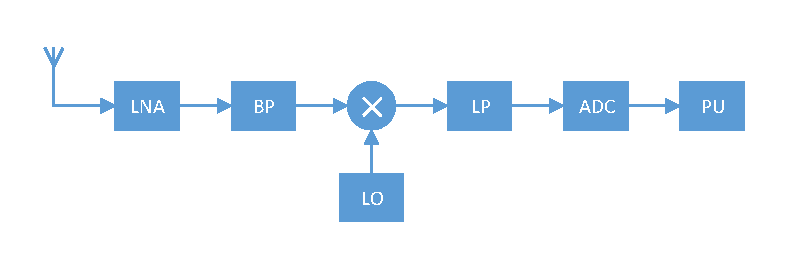
\includegraphics[width= \textwidth]{figures/Receiver.pdf}
\caption{A basic receiver structure.}
\label{fig:basic_receiver_structure}
\end{figure}

Each block will analysed with focus on the properties that could influence measurements on the fading gain i.e. gain, noise, distortion etc.

\textbf{Antenna}\\
In a line-of-sight case the received power can be expressed as \citep[p. 86]{balanis}:
%\begin{equation}
%s(t) = \int_0^{2\pi} \! \int_0^\pi G_{ant}(\theta,\phi)\cdot s(\theta,\phi,t) \,\text{d}\phi \,\text{d}\theta
%\end{equation} 
%\begin{where}
%\va{$s(t)$}{is the received signal at the antenna}{W}
%\va{$s(\theta,\phi,t)$}{is the signal strength in the $(\theta,\phi)$ direction}{W}
%\va{$G_{ant}(\theta,\phi)$}{is the gain in the $(\theta,\phi)$ direction}{1}
%\va{$\theta$}{is the azimuth angle}{rad}
%\va{$\phi$}{is the elevation}{rad}
%\end{where}

\begin{equation}
P_r(t) = \frac{D_t\cdot A_r}{4\pi\cdot R^2}\cdot P_t(t)
\end{equation} 
\begin{where}
\va{$P_r(t)$}{is the received signal at the receiving antenna}{W}
\va{$D_t$}{is the directivity of the transmitter antenna}{1}
\va{$A_r$}{is the effective area of the receiving antenna}{$m^2$}
\va{$R$}{is the distance between transmitter and receiver}{m}
\va{$P_t(t)$}{is the transmitted signal at the transmit antenna}{W}
\end{where}

It might be possible to use this to gain a extra dimension in the measurement setup, however it might also be a problem as the assumptions for the Doppler spectrum and often relies on omnidirectional reception. Normally it is possible to calibrate the system to account for gain to find the actual signal level, however it is not possible to account for an imbalance in the antenna pattern. 


Impedance mismatch typically occur where the signal is fed from the antenna to the rest of the system, this can be formulated as \citep[p. 63]{balanis}:

\begin{align}
%x_V(t) = (1+\Gamma)\cdot s_V(t) \\
%x_I(t) = (1-\Gamma)\cdot s_I(t) \\
x_P(t) = (1-|\Gamma|^2)\cdot P_r(t) \label{eq:ref_power}
\end{align}
\begin{where}
\va{$x_P(t)$}{is the power transmitted through to the system}{W}
\va{$\Gamma$}{is the reflection coefficient}{1}
\end{where}

This typically introduces both a gain and a phase distortion, however with calibration this is not an issue.

\textbf{\Gls{LNA}}\\
When the signal is passed through the LNA it can be described as:

\begin{equation}
x_{LNA}(t) = G_{LNA}\left(x_P(t)\right)*x_P(t)
\end{equation}
\begin{where}
\va{$x_{LNA}(t)$}{is the outputed signal from the LNA}{W}
\va{$G_{LNA}\left(x_P(t)\right)$}{is the gain of the LNA dependent on the input power}{1}
\end{where}

If the signal conforms to $|x_P(t)| < sat$ where sat is the saturation limit of the LNA, $G_{LNA}\left(x_P(t)\right)$ becomes a constant and the convolution becomes a multiplication, however if the power level reaches the saturation level then this is not the case and the complicated convolution is necessary. It is further not easy to calibrate for the distortion introduced by saturating the LNA.


\textbf{\Gls{BP}}\\
When the siganl is passed through a BP filter it can be described as
\begin{equation}
%x_{BP}(t) = H_{BP}(t)*\left(G_{LNA}\left(x_P(t)\right)*x_P(t)\right)
x_{BP}(t) = H_{BP}(t)*x_{LNA}(t)
\end{equation}
\begin{where}
\va{$x_{BP}(t)$}{is the signal outputted from the BP filter}{W}
\va{$H_{BP}(t)$}{is the impulse response of the BP filter}{1}
\end{where}

Implications of the BP is the signal becomes band limited which helps reduce noise, however for the filter to work it needs to settle and it also introduces a group delay. The settle time is often between $\frac{1}{f_c}$ and $\frac{3}{f_c}$%http://www.freqdev.com/guide/analog.html
but is highly dependent on the actual order of the filter. The group delay is however not easy to correct, it is therefore desirable to a linear phase shift through the filter as that introduces a constant delay to all frequencies, however in practice this is not case. 


\textbf{Mixer}\\
The mixer is the the only component that relies on its non-linearities in the chain. It takes two input namely the data caring signal and the mixing signal from the \gls{LO} a it can be modelled as \citep[p. 12]{Mixer}:
\begin{equation}
%x_{Mixer}(t) = \left(H_{BP}(t)*\left(G_{LNA}\left(x_P(t)\right)*x_P(t)\right)\right)\cdot sin\left(2\pi\cdot (f_{LO}+\epsilon_{drift}(t)) \cdot t\right)
x_{Mixer}(t) = x_{BP}(t) \cdot sin\left(2\pi\cdot (f_{LO}+\epsilon_{drift}(t)) \cdot t\right)
\end{equation}
\begin{where}
\va{$x_{Mixer}(t)$}{is the output from the mixer}{W}
\va{$f_{LO}$}{is the frequency of the LO}{Hz}
\va{$\epsilon_{drift}(t)$}{is the drift in frequency of the LO}{Hz}
\end{where}


Most of the distortion in the processed signal comes from this component, as the process is highly non-linear. The $\epsilon_{drift}(t)$ is often quite small and as long as it does not change the signal to conflict with the LP then it can typically be neglected for all intents and purposes. However a lot of extra frequency components is added to the signal due to the nature of the mixer.

%%%%%%%%%%%%%%%%%%%%%%%%%%%%%%%%%%%%%%
%%%%%%%%%%%%%%%%%%%%%%%%%%%%%%%%%%%%%%
% DO STUFF WITH THIS

%A filter needs approximately $\frac{1}{2\cdot fd_{max}}$\todo{find source (right now found from patricks mail} seconds to settle. This means a measurement should run for at least that amount of time, also the saturation can be avoided by lowering the transmit power. The frequency drift of a oscillator is typically $\pm 50ppm$ \todo{source, link is here} %$http://dk.farnell.com/webapp/wcs/stores/servlet/Search?catalogId=15001&langId=45&storeId=10157&categoryId=700000058502&pageSize=25&showResults=true$}

%%%%%%%%%%%%%%%%%%%%%%%%%%%%%%%%%%%%%%
%%%%%%%%%%%%%%%%%%%%%%%%%%%%%%%%%%%%%%

\textbf{\Gls{LP}}\\
The LP filter make sure that most of the unwanted components introduced from the mixer gets reduced significantly. It is modelled in much the same manner as the BP filter and comes with the same problems. 
\begin{equation}
%x_{LP}(t) = H_{LP}(t)*\left(\left(H_{BP}(t)*\left(G_{LNA}\left(x_P(t)\right)*x_P(t)\right)\right)\cdot \left(f_{LO}+\epsilon_{drift}(t)\right)\right)
x_{LP}(t) = H_{LP}(t)*x_{Mixer}
\end{equation}
\begin{where}
\va{$x_{LP}(t)$}{is the outputted from the LP filter}{W}
\va{$H_{LP}(t)$}{is the impulse response of the LP filter}{1}
\end{where}

The settle time of the LP is often magnitudes longer than the settle time of the BP as the frequencies involved are much lower. 

After this the \gls{ADC} quantise and digitalize the signal so a \gls{PU} can process it. Through this analysis different parameters have been found to affect the signal in the receiver, ending in a rather complicated expression. If an network analyser is used for measurement then most of these problems is dealt with, in a way that makes it of little concern e.g. the signal never saturates the amplifiers the drift in the LO is measured and accounted for etc. The rest of the distortion introduced can be calibrated as it is deterministic. 


%
%
%
%%These problems can be categorized into what can be accounted for during the measurement, what can be accounted for by calibrating the equipment and what can not be easily dealt with.
%%
%\begin{itemize}
%\item Avoidable problems
%	\begin{itemize}
%	\item Settle time
%	\item Saturation
%	\end{itemize}
%\item Calibration problems
%	\begin{itemize}
%	\item Reflection
%	\item Gains
%	\end{itemize}
%\item Distortion problems
%	\begin{itemize}	
%	\item Phase shift/ group delay
%	\item Drift
%	\item Non-linearities
%	%\item Effective number of bits
%	\end{itemize}
%%\item Statistical problems
%%	\begin{itemize}
%%	\item Noise
%%	\item Quantization noise
%%	\end{itemize}
%\end{itemize}
%%
%Parameters that is critical to the measurements is the BW and the antenna pattern as these two directly influence the measurement of the channel. The rest only has indirect implications on the measurements. This is supported by related work in \citep{MeasurementComplexRay}
\textbf{Noise}\\
A problem that has not been addressed is the noise aspect, all components in the receiver chain produces noise. Normally the figure of interest is the noise power a typical model for the noise power is a Gaussian process. As this process is a random process the noise can not be accounted for by calibration as with the distortion. Furthermore the Rayleigh fading model is a complex Gaussian process which means that it can be next to impossible to distinguish between the contribution from fading and noise in the received signal. Based on these arguments it is assumed that noise is the dominant factor which needs to be accounted for where the distortion introduced by the components will be less and in most cases reduced further by calibration.


\section{Dynamic range}
Dynamic range in RF systems is the ability of the receiver to pick out weak signals compared to the strong ones(the range of the low signals to the high signals which the receiver can operate). Think about it as trying to hear a person talking when somebody in the room is screaming.  
With manual or automatic gain control,the total dynamic range of the receiver will allow it to accept a wider range of signal power.That isn't a problem as long as we want to observe the strongest signal or nearly the strongest one.The situation gets tricky when we want to observe a really weak signal in the presence of much stronger ones.That is the point where we are more interested in the instantaneous dynamic range.
The instantaneous dynamic range is specified as the difference between the strongest to the weakest signal(in dB) that can be present in a receiver's pass band while the receiver is meeting full specified performance in receiving and processing the weaker signal.
The maximum strength that a receiving system can accept and process depends on the sensitivity of the receiver and it's dynamic range.
\begin{equation}
MAXstr_{dBm} = (Sens) +(DR)
\label{Max strength of a receiving system}
\end{equation}

Where $MAX_{str}$ is the maximum strength of a receiving system,Sens is the sensitivity of the receiver and DR the dynamic range of the system.\citep{DyR}

Receiver sensitivity is defined as the weakest signal that can be observed and still provide a sufficient quality output.Sensitivity is determined by the sum of Thermal Noise ,Noise Figure and the Required prediction of SNR.It is normally a negative number(in dBm) and this means that a bigger number(more negative) equals a smaller signal.
The thermal noise is given by:
\begin{equation}
Noise_{dBm} = 10log(BW\cdot Te\cdot k\cdot 1000) + NF
\label{Noise1}
\end{equation}
where $BW$ is the bandwidth $Te$ is the thermal temperature and the $NF$ is the noise figure of the reviver.

Dynamic Range or else Signal to noise and Distortion Ratio(SINAD) is also very similar to the Signal to Noise Ratio(SNR). SINAD is a good way to describe the whole dynamic system of ADC because takes into account all the components that make noise and distortion,in other words takes into account the non-linearities. The difference between them can be shown in high frequencies because the SINAD gets affected by the distortions and degrades faster than the SNR that excludes the first 5 harmonics that are dominant.The clear difference can be shown from the two formulas:
\begin{equation}
\text{SINAD} = 20log\left(\frac{S}{N+D}\right)
\end{equation}

\begin{equation}
\text{SNR} = 20log\left(\frac{S}{N}\right)
\end{equation}
where S represents the signal power,N the Noise and D the Distortion.\citep{SINADandSNR}
\subsection{SNR margin estimation}
\label{SNR_margin}
Because the noise might influence the deep fades of our signal, a minimum SNR margin needs to be estimated.
This gives us the SNR margin needed to distinguish a deep fade from the noise floor. % given a set confidence interval and margin.
%By doing this gives we will be able to accept the measurements that are above this margin and reject the ones that are affected by the noise.
The estimation assume the signal as a constant and the noise as a complex vector that changes. Therefore a Rician distribution can be used, because it consists of constant part and random part.
\begin{equation}
p = a^2 + 2\sigma^2
\end{equation}
\todo {change symbols}
Rician distribution fits in this situation because the K-factor that it depend upon is a ratio of power for the constant signal to the random noise, \citep{SpaceWirelessChan} meaning that the K-factor matches the SNR margin that we need to estimate.
\begin{equation}
K = \frac{a^2}{2\sigma^2}
\end{equation}
Given that we set our confidence interval of $\pm 1$dB around the value of our constant signal in the Rician cdf matched with the 90\% confidence level on the probability axis, we are able to estimate numerically the part of the K-factor that we are interested in.
\begin{figure}[H]
\centering
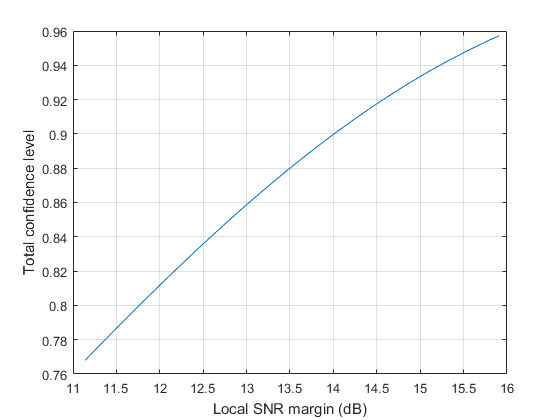
\includegraphics[width=0.70\textwidth]{figures/SNR_margin.png}
\caption{Solving for the K-factor numerical gives a estimate of SNR Margin. At 0.90 confidence with $\pm 1$dB margin  the K-factor is 14dB.}
\label{Rician_90}
\end{figure}

The results show that a SNR margin $SNR_m$ of 14dB is needed to have accurate reading of the deep fades.
The total dynamic range requirement becomes:
\begin{equation}
DR_{tot} = SNR_m - G_f , 14dB + 50dB = 64dB 
\end{equation}
\begin{where}
\va{$DR_{tot}$}{Total dynamic range}{dB}
\va{$SNR_m$}{is the SNR margin }{dB}
\va{$G_f$}{is the fading gain we want to measure (-50dB)}{dB}
\end{where}



\subsection{How to measure dynamic range}

In a normal receiver the dynamic range is set by the sensitivity of the receiver to the Third order intercept point. Third order intercept points are caused by over driving the receiver with too much input and that causes distortion and signal saturation. The sensitivity is more dependent on the operating environment and the receivers noise figure. \citep{understandDynamic}


\begin{figure}[H]
\centering
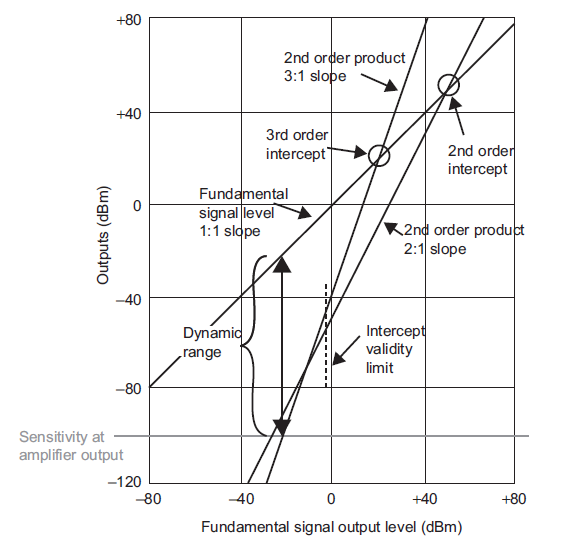
\includegraphics[width=0.90\textwidth]{figures/Dynamic_range_calc.png}
\caption{Determining the Dynamic Range from the spurs and sensitivity line.(WORK IN PROGRESS!!)}
\label{Dynamic_range_calc}
\end{figure}
 
This means that a RF receiver is highly dependent on the mixer and amplifier with regards to dynamic range. A measurement system would take into account the factors listed in \autoref{basic_rev_struct} to increase the dynamic range. Going through the \autoref{fig:basic_receiver_structure} in order from left to right. The receivers \gls{IF} is the frequency that shifted to in order to process the signal easier.  This is done in the first stages of a receiver. This frequency is normally lower than the transmitted RF frequency, this especially helps the \gls{ADC} that uses a lower sampling rate. 
By setting the \gls{IF} filter to a very narrow bandwidth (narrowband) the noise floor goes down and increases the dynamic range. 

\section{Time to do a sweep}
The cost of using a narrowband is the measurement time, as the system would require a longer time for the sweep to cover a typical bandwidth. The time this would take is given by:
\todo{maybe write about averaging here and add it to the Time calculations}
\begin{equation}
T = \frac{1}{IF_{BW}} \cdot \frac{BW_{sweep}}{IF_{BW}}
\end{equation}
where $IF_{BW}$ is the intermediate frequency bandwidth and $BW_{sweep}$ is the total bandwidth you want to measure.


\subsection{Dynamic range in a VNA receiver}
\begin{figure}[H]
\centering
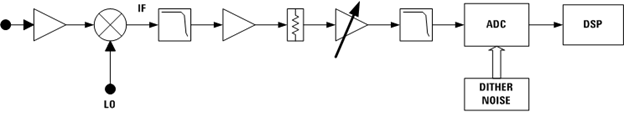
\includegraphics[width=0.90\textwidth]{figures/Block_VNA.png}
\caption{A Typical block diagram of a VNA receiver.}
\label{Block_VNA}
\end{figure}

For Network analysers the dynamic range is the maximum signal power the receiver can measure minus the noise floor of the receiver. To achieve a higher dynamic range of \gls{VNA} it must be  in tuned-receiver mode (Narrowband).
If you reduce the bandwidth then the overall noise floor will go down, so it logical that it would have higher dynamic range. \citep{AgilentNVA} \\
%%The setup of the \gls{VNA} measuring would have to take into account some factors to increase the dynamic range and still have the accuracy. Going through the \ref{Block_VNA} in order from left to right.
%%The \gls{IF} is a frequency that shifted to in order to process the signal easier. This is done in the first stages of a receiver. This frequency is normally lower than the transmitted RF frequency, this especially helps the \gls{ADC} that uses a lower sampling rate. 
%%By setting the \gls{IF} filter to a very narrow bandwidth (narrowband) the noise floor goes down and increases the dynamic range. The cost of using a narrowband is the measurement time, as the \gls{VNA} would need several sweeps to cover a typical bandwidth. \\

Dynamic range and accuracy are affected by the non-linearity in the receiver chain, the worst part are the mixers,\gls{ADC} and amplifiers since they introduce the most non-linearity. To measure the linearity of a receiver a power change measurements is preformed and compared to a reference level of power change that is accurate. This means that the linearity of a receiver as can be defined as:
\begin{equation}
Linearity = \frac{receiver \\\ measured \\\ power \\\ change}{reference \ power \ change}
\label{Linearity}
\end{equation}
 

Cross talk is the energy leakage between signal paths of the measuring system and it can be a problem in high-loss transmission measurements. This can be fixed by running an isolation calibration \citep{crosstalk}.It occurs below the noise floor so averaging and low \gls{IF} filter bandwidth must be used during calibration.
At low power levels <-70dBm the main non-linearity comes from the \gls{ADC}. Quantizing error occurs when converting from analog to digital signals. The \gls{ADC} used in \gls{VNA} are top of the line and can use a Gaussian noise ditcher to combat the non linear nature of a \gls{ADC}. 


In the digital signal processing of the \gls{VNA} averaging be applied to reduce the noise.Given the noise is uncorrelated, by averaging the measured(complex) data the noise component will approach zero.That means that our end signal in the output will be with less noise.Every time that our average is getting doubled, the signal to noise ratio is increased by 3dB. The problem is that by averaging the double of every data point the measurement will take twice as long.\citep{KeysightAVG}. The total noise floor is then given by:

\begin{equation}
Noisefloor_{dBm} = log_{2}(AVG_f)\cdot 3dB +10log(IF_{BW}\cdot T_{0}\cdot k\cdot 1000) + NF 
\label{NFwithAVG}
\end{equation}
Where $IF_{BW}$ is  intermediate bandwidth $T_0$ is temperature of the system, $k$ is the Boltzmann's constant,$AVG$ is the averaging factor and $NF$ if the noise figure.
To maximise the effectiveness of a \gls{VNA} the reviver $IF_{BW}$ should be high as possible for the dynamic range needed. So to get accurate samples with the needed dynamic range in the least amount of time the $IF_{BW}$ and $AVG_f$ must be balanced to minimise time spent on one measurement.
Equipment drift is another source of error that can occur if we are operating in a place with different environmental factors for a long period of time.


%\section{Diversity}
%% (effects?)
%Diversity is used to combat fading in a wireless system. By using clever techniques you can effectively deliver several copies or replicas of a signal to the receiver. There is a lower chance that all of these copies of signals are going to have a deep fade at the same time \citep[p. 4-6]{diversityFuture}. The overall goal is to provide a gain in signal quality by having several signals that independently fade from each other without the cost of more power consumption, reduced bit rate and complexity or other resources. There are several ways to achieve diversity in a wireless system. \\
%Time diversity: By retransmitting the same information you get some diversity gain on the cost of decreased bit/rate. Usually a forward error correction code is added instead of just re transmitting the signals several times. \\
%Antenna diversity / Spatial diversity
%By having several antennas at both/or the receiver and transmitter a antenna diversity is achieved. With several antennas the signal can be combined together to process the signals into one. To get independently fading signals the signals need to be uncorrelated by separating the antennas least half a wavelength (micro diversity) \citep{diversityAntenna}. Antenna diversity comes at the cost of having to power more than one antenna.


\subsection{How to measure uncorrelated samples}
\label{howtomeasureUS}
To measure the required samples from \autoref{sampleEQ} ($\approx 4.04\cdot10^6$) uncorrelated samples requires a elaborate test setup. The limitation is in how much space and time the measurement is going to require. The total number of samples that can be obtained can be expressed as: 
\todo {removed big part here, maybe move it to measurement setup}
%The example scenario  will have a $f_c$ of 3Ghz, BW of 100MHz, a $5x5$ antenna array, a office building with a delay spread of 100ns and a room size that is $10m \cdot 10m$.
%If we assume we have a multipath delay spread of 100ns. Given \autoref{CohBW} the $B_C$ is 1.6MHz. Since the $B_C$ is only a approximation with some coherence, the $B_C$ should be increased to approximate 3 Mhz to get less correlated samples. This will give round 30 uncorrelated samples in frequency with a BW of 100MHz.
%The $f_c$ of 3Ghz gives a $\lambda$ of 0.1m or 10cm. The array antennas has each antenna spaced half a $\lambda$ which would give a total antenna length of 0.25m. If the antenna array is moved in one dimension,every step needs to be spaced $0.25+\frac{\lambda}{2}$ apart. Given the 10m size of the room 30 samples is possible in 1 dimension. If the measurements is done in 2 dimensions ($10m\cdot 10m$) a total area of:

\begin{equation}
N = \underbrace{A_{div}}_\text{$N_a$} \cdot \underbrace{\frac{BW}{B_c \cdot 2}}_\text{$N_f$} \cdot \underbrace{\frac{\Delta}{(\frac{\lambda}{2})^2}}_\text{$N_d$}
\label{howtosample}
\end{equation} 
 
\begin{where}
\va{$N$}{Total samples}{1}
\va{$N_a$}{parallel antenna samples}{1}
\va{$N_f$}{samples in frequency}{1}
\va{$N_d$}{samples in space}{1}
\va{$A_{div}$}{antenna diversity}{1}
\va{$\Delta$}{is the area }{$m^2$}
\va{$B_c$}{is the coherence BW }{Hz}
\va{$\lambda$}{wavelength}{m}
\end{where} 
 
%Where $N$ is number of samples(in antenna diversity,frequency and space), $A_{div}$ is the antenna diversity, $\Delta$ is the area, $B_c$ is the coherence BW and $\lambda$ is the wavelength.

\autoref{howtosample} can be used to found the area required given number of samples $N$ needed.

\begin{equation}
\Delta  = \frac{N\cdot (\frac{\lambda}{2})^2}{A_{div}\cdot \frac{BW}{B_c \cdot 2}}
\label{howtosqaure}
\end{equation}

If the area of the measurement is not big enough to take all the measurements different rooms could be used. To do this you need to normalize for the mean gain the system sees. It's clear that taking $4.04\cdot10^6$  uncorrelated samples requires taking advantage of  frequency(bandwidth),space or time to get the necessary samples. The best way is to balance and connect these values to the limitation in the equipment and measurement setup. This will be examined in later sections. 
%If we assume a $10m \cdot 10m$ this gives us: 
%\begin{equation}
%\frac{10m}{\frac{\lambda}{2}} \cdot \frac{10m}{\frac{\lambda}{2}}  = 40000 samples
%\end{equation}
%The total amount of spatial, frequency and antenna array uncorrelated samples is:
%\begin{equation}
%30 \cdot 25 \cdot 40000 = 3 \cdot 10^7 samples
%\end{equation}
%which is way more then we need.
%Actually moving the reviver $2 \cdot 10^6$ times takes way to long to actually do, but this example calculation is just to show that it is possible to obtain $10^7$ samples.If the area of the measurement is not big enough to take all the measurements different rooms could be used. To do this you need to normalize for the mean gain the system sees. 

A other problem with a taking $4.04\cdot10^6$  uncorrelated samples is that the channel may be changing because of frequency shift or movement. This will make the samples uncorrelated, but you are in danger of measuring a completely different channel. Here comes the non-stationary principle into play. A argument could be made that the $10^{-5}$ fading is so dependant on the environment that a measurement would only be valid for this exact room or situation you are measuring.

\subsection{Time required to do measurements}
\todo{Write more general or remove/move to part II}
When trying to obtain a high number of samples, time becomes a very limiting factor. For this reason a estimation of total measurement time or a time budget is helpful. If one sample takes 1 second to measure and the required samples size is $10^7$, the total measuring time would be 116 days of continues measurements. This of course is not practical to do. So it's obvious that a automatic systems that takes several samples in parallel is needed. The time budget uses the values from  \autoref{howtomeasureUS} and assumes the samples are measured continuously in one dimension with a velocity of $1m/s$. 
The antenna array is spaced in a different dimension so samples don't overlap. The time it would take to do a $100MHz$ sweep is dependant on the $IF_{BW}$ and dynamic range requirements discussed later. The calculation assumes that system can do a full sweep over the BW at every $\frac{\lambda}{2} = 0.05m$ and get the 30 samples in frequency or $N_f$. So first lets calculate the amount of samples we can do per second $N_s$:
\begin{equation}
N_s = \frac{v}{\frac{\lambda}{2}}\cdot N_f \cdot A_{div}, \frac{1m/s}{0.05m} \cdot 30N \cdot 25N = 15000N_s
\end{equation}
Then the total time needed for a continues measurements:
\begin{equation}
T = \frac{N}{N_s} , \frac{10^7N}{15000N_s} = 667s \approx 12 minutes.
\end{equation}
The total time budget shows that multiple uncorrelated samples must be acquired at a relative high speed in order to get the needed sample size. A speed of $1m/s$ over 12 minutes is equal to $720m$ in one dimensions so a two dimensional space separation is needed to reduce the room size requirement.. The practicality of this will be discussed in part II.
%\section{Introduction of noisy signal}
